\documentclass[cjk,slidestop,compress,mathserif,blue]{beamer}
%dvipdfm选项是关键,否则编译统统通不过
%beamer的颜色选项定义的是导航条和标题的颜色(即关键词structure的颜色)

%%%%%%%%%%%%%%%%仅限于XeTeX可使用的宏包%%%%%%%%%%%%%%%%%%%%%%%%%%%%
\usepackage{fontspec,xunicode,xltxtra,beamerthemesplit}
%\usepackage{beamerthemesplit}
\usepackage{xeCJK}
\setCJKmainfont[BoldFont=黑体, ItalicFont=楷体, BoldItalicFont=仿宋]{黑体}
%\setsansfont[Mapping=tex-text]{Adobe 黑体 Std}
%如果装了Adobe Acrobat,可在font.conf中配置Adobe字体的路径以使用其中文字体
%也可直接使用系统中的中文字体如SimSun,SimHei,微软雅黑 等
%原来beamer用的字体是sans family;注意Mapping的大小写,不能写错

%%%%%%%%   确定标题和导航条结构的框架     %%%%%%%%%%%%
\usepackage{beamerthemeshadow}                       %
%\usepackage{beamerthemeclassic}%导航条色与背景色一致%
%%%%%%%%%%%%%%%%%%%%%%%%%%%%%%%%%%%%%%%%%%%%%%%%%%%%%%
\setbeamerfont{roman title}{size={}}
%\usepackage{CJK} % CJK 中文支持                                  %
\usepackage{amsmath,amsthm,amsfonts,amssymb,bm}
\usepackage{mathrsfs}
\usepackage{xcolor}                                        %使用默认允许使用颜色
\usepackage{hyperref} 
\usepackage{graphicx}
\usepackage{subfigure}           %图片跨页
\usepackage{animate}		 %插入动画

%\usepackage[numbers,sort&compress]{natbib} %紧密排列             %
\usepackage[sectionbib]{chapterbib}        %每章节单独参考文献   %
\usepackage{hypernat}                                                                         %
%\usepackage[dvipdfm,bookmarksopen=true,pdfstartview=FitH,CJKbookmarks]{hyperref}		%
\hypersetup{bookmarksnumbered,colorlinks,linkcolor=brown,citecolor=blue,urlcolor=red}         %
%参考文献含有超链接引用时需要下列宏包,注意与natbib有冲突        %
%\usepackage[dvipdfm]{hyperref}                                  %
%\usepackage{hypernat}                                           %
\newcommand{\upcite}[1]{\hspace{0ex}\textsuperscript{\cite{#1}}} %

%\useoutertheme{smoothbars}
\useinnertheme[shadow=true]{rounded}
\usetheme{Berkeley}                                          %主题式样
%\usetheme{Luebeck}

\usecolortheme{lily}                                        %颜色主题式样

\usefonttheme{professionalfonts}                           %字体主题样式宏包

%\beamertemplatetransparentcoveredhigh                      %使所有被隐藏的文本高度透明
\beamertemplatetransparentcovereddynamicmedium             %使所有被隐藏的文本完全透明,动态,动态的范围很小
\mode<presentation>
%\beamersetaveragebackground{gray}                          %设置背景颜色(单一色) 
\beamertemplateshadingbackground{green!10}{red!5}         %设置背景颜色(渐变色)

%在指定位置精确放置logo
\usepackage{tikz}
\usepackage{beamerfoils}
\usepackage{pgf}
\logo{\pgfputat{\pgfxy(11.68,0.15)}{
\includegraphics[height=1.01cm,viewport=0 0 140 120,clip]{Figures/BCC_logo-1.png}}\pgfputat{\pgfxy(10.502,-0.218)}{
\includegraphics[height=0.369cm,viewport=140 0 540 120,clip]{Figures/BCC_logo-1.png}}}
%\logo{\pgfputat{\pgfxy(11.68,0.15)}{
\includegraphics[height=0.95cm,viewport=0 0 510 360,clip]{Figures/Logo_Gainstrong.png}}\pgfputat{\pgfxy(10.333,-0.195)}{
\includegraphics[height=0.35cm,viewport=530 70 1100 218,clip]{Figures/Logo_Gainstrong.png}}}
%\MyLogo{
%	\pgfputat{\pgfxy(-50,-50)}{\pgfbox[right,base]{
\includegraphics[height=1cm]{Figures/BCC_logo-1.png}}}

%logo作为背景放置
%\setbeamertemplate{background}{
%	\pgfputat{\pgfxy(6.5,-0.5)}{\pgfbox[left,top]{\pgfimage[height=1.1cm]{Figures/BCC_logo-1.png}}}}

%\logo{}									%不显示logo

\begin{document}
%\begin{CJK*}{GBK}{song}
%\begin{CJK*}{GBK}{kai}
%beamer下不能用\songyi、\zihao等命令!
%\graphicspath{Figures/}

%-------------------------------PPT Title-------------------------------------
\title{量子力学基础:~Hartree-Fock}
%-----------------------------------------------------------------------------

%----------------------------Author & Date------------------------------------
\author{北京市计算中心\;云平台\:姜骏}
\date{\textrm{2016.08.22}}
%\date{2013.09.10}
\frame{\titlepage}
%-----------------------------------------------------------------------------

%------------------------------------------------------------------------------列出全文 outline ---------------------------------------------------------------------------------
\section*{}
\frame[allowframebreaks]
{
  \frametitle{Outline}
%  \frametitle{\textcolor{mycolor}{\secname}}
  \tableofcontents%[current,currentsection,currentsubsection]
}
%在每个section之前列出全部Outline
%类似的在每个subsection之前列出全部Outline是\AtBeginSubsection[]
\AtBeginSection[]
{
  \frame<handout:0>
  {
    \frametitle{Outline}
%全部Outline中,本部分加亮
    \tableofcontents[current,currentsection]
  }
}

%------------------------------------------------------------------------------PPT main Body------------------------------------------------------------------------------------
\small
\section{量子力学基本假设}
\frame
{
	\frametitle{量子力学的奠基人}
\begin{figure}[h!]
\centering
\vspace{-25.5pt}
\hspace*{-15.5pt}
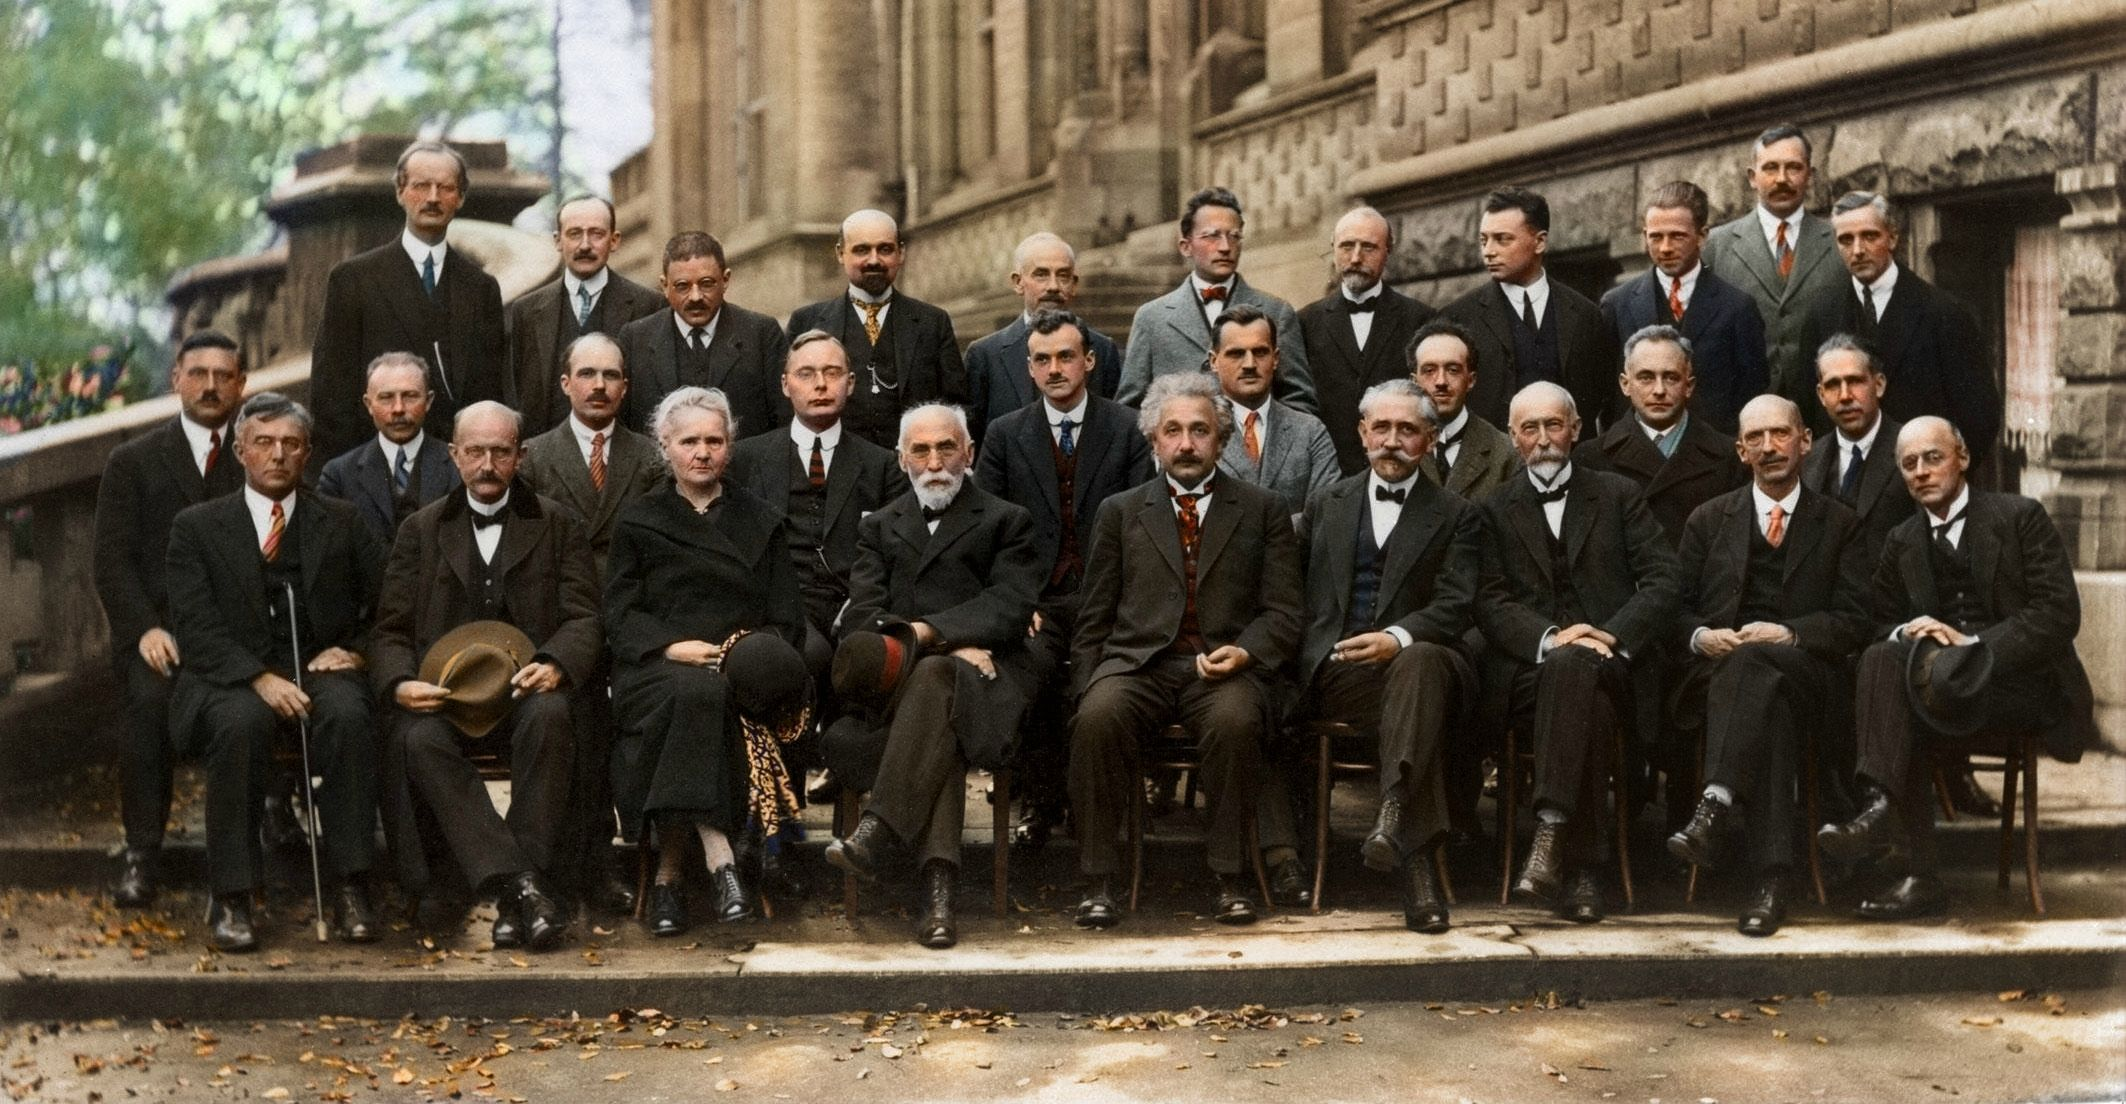
\includegraphics[height=0.57\textwidth,width=1.1\textwidth,viewport=0 0 2150 1050,clip]{Figures/Solvay_Conference-5-fine.jpg}
\caption{\fontsize{7.5pt}{6.2pt}\selectfont{\textrm{The Fifth Solvay International Conference, Brussels, Belgium, Oct. 1927}}\\
\fontsize{4.1pt}{3.9pt}\selectfont{\textrm{\textcolor{blue}{前排左起}:~I.Langmuir(\textcolor{blue}{朗缪尔}) M.Planck(\textcolor{blue}{普朗克}) Marie Curie(\textcolor{blue}{居里夫人}) H.Lorentz(\textcolor{blue}{洛仑兹}) A.Einstein(\textcolor{blue}{爱因斯坦}) P.Langevin(\textcolor{blue}{朗之万}) Ch.E.Guye(\textcolor{blue}{古伊}) C.T.R.Wilson(\textcolor{blue}{威尔逊}) O.W.Richardson(\textcolor{blue}{理查森})\\
\textcolor{blue}{中排左起}:~P.Debye(\textcolor{blue}{德拜}) M.Knudsen(\textcolor{blue}{克努森}) W.L.Bragg(\textcolor{blue}{布拉格}) H.A.Kramers(\textcolor{blue}{克莱默}) P.A.M.Dirac(\textcolor{blue}{狄拉克}) A.H.Compton(\textcolor{blue}{康普顿}) L.de Broglie(\textcolor{blue}{德布罗意}) M.Born(\textcolor{blue}{玻恩}) N.Bohr(\textcolor{blue}{玻尔})\\
\textcolor{blue}{后排左起}:~A.Piccard(\textcolor{blue}{皮卡尔德}) E.Henriot(\textcolor{blue}{亨利厄特}) P.Ehrenfest(\textcolor{blue}{埃伦费斯特}) Ed.Herzen(\textcolor{blue}{赫尔岑}) Th.de Donder(\textcolor{blue}{德唐德}) E.Schr\"odinger(\textcolor{blue}{薛定谔}) E.Verschaffelt(\textcolor{blue}{费尔夏费尔特}) W.Pauli(\textcolor{blue}{泡利}) W.Heisenberg(\textcolor{blue}{海森堡}) R.H.Fowler(\textcolor{blue}{富勒}) L.Brillouin(\textcolor{blue}{布里渊})}}}
\label{Solvay Conference-5-fine}
\end{figure}
}
%------------------------------------------------------------------------Reference----------------------------------------------------------------------------------------------
\frame
{
	\frametitle{量子力学基本假设}
	\begin{itemize}
		\item 波函数假定\\
			\textcolor{blue}{微观体系的运动状态可由波函数$\Psi$完全描述,波函数可以得到体系的所有性质}\\
			波函数$\Psi$一般要求满足\textcolor{red}{连续}、\textcolor{red}{有限}和\textcolor{red}{单值}三个条件

		\item 力学量算符假定\\
			\textcolor{blue}{力学量用线性\textrm{Hermite~}算符表示}\\
			在经典力学中的力学量,在量子力学中用力学量的算符表示:\\如动量算符 
			$$\hat{\mathbf{p}}=-\mathrm{i}\hbar\nabla$$
			位置算符$$\hat{\mathbf r}=r$$
			力学量算符\textcolor{red}{有组成完全系的本征函数}
	\end{itemize}
}

\frame
{
	\frametitle{量子力学基本假设}
	\begin{itemize}
%		\item 力学量算符之间有确定的对易关系(量子条件)
%			$$[\hat{\mathbf F},\hat{\mathbf G}]=\hat{\mathbf F}\hat{\mathbf G}-\hat{\mathbf G}\hat{\mathbf F}$$ 
		\item 态叠加原理\\
			如果$\Psi_1$是体系的一个本征态,对应的本征值为$A_1$,$\Psi_2$也是体系的一个本征态,对应的本征值为$A_2$,则\textcolor{blue}{$$\Psi=C_1\Psi_1+C_2\Psi_2$$}\textcolor{red}{也是体系一个可能的存在状态}
		\item 微观体系的运动状态\textcolor{blue}{波函数随时间变化的规律}:\\\textcolor{red}{遵从\textrm{Schr\"odinger}方程}
			$$\mathrm{i}\hbar\dfrac{\mathrm{d}}{\mathrm{d}t}|\Psi\rangle=\hat{\mathbf H}|\Psi\rangle$$
		\item 全同性原理\\
			\textcolor{blue}{全同粒子组成的体系中,两个全同粒子相互调换不改变体系的状态}\\ 
			全同粒子是指\textcolor{red}{内禀性质完全相同的一类微观粒子}:\\例如所有的电子是全同粒子 
	\end{itemize}
}

\frame
{
	\frametitle{Schr\"odinger's cat}
\begin{figure}[h!]
\centering
\vspace{-10.5pt}
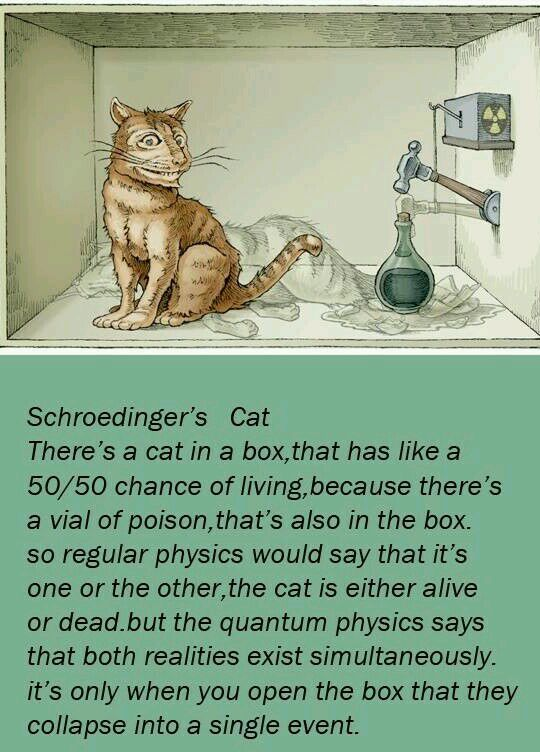
\includegraphics[height=0.70\textwidth,width=0.7\textwidth,viewport=0 0 760 750,clip]{Figures/Schrodinger-cat.jpg}
%\caption{\textrm{ABINIT}的Si.in}
\label{Schrodinger-cat}
\end{figure}
}

\section{Hartree-Fock方法}
\frame
{
	\frametitle{Born-Oppenheimer近似}
	\begin{itemize}
		\item 由于原子核的质量要比电子大很多(一般要大3-4个数量级),在同样的相互作用下,原子核的运动比电子也慢得多
		\item 电子在每一时刻仿佛运动在静止原子核构成的势场中,而原子核运动时则感受不到电子的具体位置,感受到的是运动电子的平均作用力
		\item 可近似将原子核坐标与电子坐标变量分离,使得求解整个体系的波函数的复杂过程分解为求解电子波函数和求解原子核波函数两个相对简单的过程\\
			电子运动方程$$\hat{\mathbf H}_{\mathrm e}(\vec r,\vec{\mathbf R})\Psi(\vec r,\vec{\mathbf R})=E_{\mathrm e}(\vec{\mathbf R})\Psi(\vec r,\vec{\mathbf R})$$
			原子核运动方程$$[\hat{\mathbf T}_{\mathrm{nul}}+E_{\mathrm e}(\vec{\mathbf R})]\chi(\vec{\mathbf R})=E\chi(\vec{\mathbf R})$$
	\end{itemize}
}

\frame
{
	\frametitle{独立粒子近似}
	\textrm{n-}粒子体系中的每个粒子的运动,完全忽略粒子间的瞬时相互作用,认为第$i$个粒子在其余$\mathrm{n}-1$个粒子组成的平均势场中运动
	$$\Psi(\vec r_1,\vec r_2,\vec r_3,\cdots,\vec r_n)=\psi_1(\vec r_1)\psi_2(\vec r_2)\psi_3(\vec r_3)\cdots\psi_n(\vec r_n)$$
	$$\hat{\mathbf H}=\sum_{i=1}^N-\dfrac{1}{2}\nabla_i^2+\sum_{i=1}^NV_i(\vec r_i)+\sum_{i,j(j\neq i)}\dfrac{e^2}{|\vec r_i-\vec r_j|}$$
	粒子$i$的\textrm{Hartree}算符
	$$\hat{\mathbf h}_i=-\dfrac{1}{2}\nabla_i^2+V_i(r_i)+\sum_{j(j\neq i)}^N\dfrac{e^2}{|\vec r_i-\vec r_j|}$$
	因此每个粒子的运动方程为:
	$$\hat{\mathbf h}_i\psi_i(\vec r)=\bigg[-\dfrac{1}{2}\nabla_i^2+V_i(r_i)+\sum_{j(j\neq i)}^N\dfrac{e^2}{|\vec r_i-\vec r_j|}\bigg]\psi_i(\vec r)=\varepsilon\psi_i(\vec r)$$ 
}

\frame
{
	\frametitle{Slater行列式}
	简单乘积的独立粒子波函数不满足全同粒子置换对称性要求,不能正确表示电子不可辨认的物理属性
	
	\textrm{Slater}建议用行列式形式表示具有反对称性的波函数
	\begin{displaymath}
		\hspace*{-10pt}\Psi(\vec r_1,\vec r_2,\vec r_3,\cdots,\vec r_n)=\dfrac1{\sqrt{n!}}
		\left|\begin{array}{ccccc}
			\psi_1(\vec r_1)&\psi_2(\vec r_1)&\psi_3(\vec r_1)&\cdots&\psi_n(\vec r_1)\\
			\psi_1(\vec r_2)&\psi_2(\vec r_2)&\psi_3(\vec r_2)&\cdots&\psi_n(\vec r_2)\\
			\psi_1(\vec r_3)&\psi_2(\vec r_3)&\psi_3(\vec r_3)&\cdots&\psi_n(\vec r_3)\\
			&&&\cdots&\\
			\psi_1(\vec r_n)&\psi_2(\vec r_n)&\psi_3(\vec r_n)&\cdots&\psi_n(\vec r_n)
		\end{array}\right|
	\end{displaymath}
	粒子$i$的\textrm{Fock}算符
	$$\hat{\mathbf F}_i=-\dfrac{1}{2}\nabla_i^2+V_i(r_i)+\hat{\mathbf J}_i-\hat{\mathbf K}_i$$
	$$\hat{\mathbf J}_i(\vec r_i)=\int\dfrac{\psi_j^{\ast}(\vec r_j)|e^2|\psi_j(\vec r_j)}{|\vec r_i-\vec r_j|}\mathrm{d}\vec r_j$$
	$$\hat{\mathbf K}_i(\vec r_i)\psi_i(\vec r_i)=\psi_j(\vec r_i)\int\dfrac{\psi_j(\vec r_j)|e^2|\psi_i(\vec r_j)}{|\vec r_i-\vec r_j|}\mathrm{d}\vec r_j$$

}

\frame
{
	\frametitle{Hartree-Fock-Roothan方法}
	实际求解非相对论的\textrm{Schr\"odinger}方程时,
	$$\hat{\mathbf F}_i\psi_i(\vec r_i)=\varepsilon_i\psi_i(\vec r_i)$$
	将波函数$\psi_i(\vec r_i)$用一套选定的基函数$\phi_j(\vec r)$展开
	$$\psi_i(\vec r)=\sum_{j=1}^Nc_{ij}\phi_j(\vec r)$$
	通过变分原理
	$$\bar E=\dfrac{\langle\Psi|\hat{\mathbf H}|\Psi\rangle}{\langle\Psi|\Psi\rangle}\geqslant E_0$$
	改变展开系数$c_{ij}$直到体系的能量最小,确定展开系数

	重复上述流程直至\textrm{Fock}算符$\hat{\mathbf F}$、波函数$\psi(\vec r)$和能量$\varepsilon$自洽,这就是\textrm{Hartree-Fock-Roothan}方法
}

\frame
{
	\frametitle{RHF与UHF} 
	\begin{itemize}
		\item \textrm{RHF}:\\
			针对闭壳层(\textrm{closed shell})体系,占据轨道的电子成对出现,自旋相反,可用一个\textrm{Slater}行列式表示\\
	%		每对自旋相反的电子有相同的轨道波函数\\
			对于闭壳层体系,\textrm{Hartree-Fock}方法求解的能量本征值符合\textrm{Koopmans}定理
			$$E_{ion}^1=-\varepsilon_{\mathrm{HOMO}}$$
		\item \textrm{UHF}:\\
			针对开壳层(\textrm{open shell})体系,占据轨道有未成对电子,需要用\textrm{Slater}行列式的线性组合表示\\
			最低能态用一个\textrm{Slater}行列式,但不同自旋的轨道分别处理
		$$E_{\mathrm{UHF}}\leqslant E_{\mathrm{RHF}}$$
			由于\textrm{UHF}包含更多的变分函数,可以处理一些近解离极限的分子体系
	\end{itemize}
}

\frame
{
	\frametitle{交换与相关}
	\begin{itemize}
		\item \textrm{Fock}算符中的交换算符$\hat{\mathrm K}_i(\vec r_i)$是由\textrm{Slater}行列式引入的,属于量子效应
	\end{itemize}
%	\vspace*{-5pt}
	\begin{displaymath}
%		\hspace*{-2pt}
		\text{电子间瞬时相互作用(\textcolor{red}{关联})}
		\left\{
			\begin{aligned}
				&\text{\textcolor{blue}{电子交换}:同自旋电子的关联作用}\\
				&\text{\textcolor{blue}{电子相关}}
			\end{aligned}
			\right.
	\end{displaymath}
\begin{figure}[h!]
\centering
\vspace{-10.5pt}
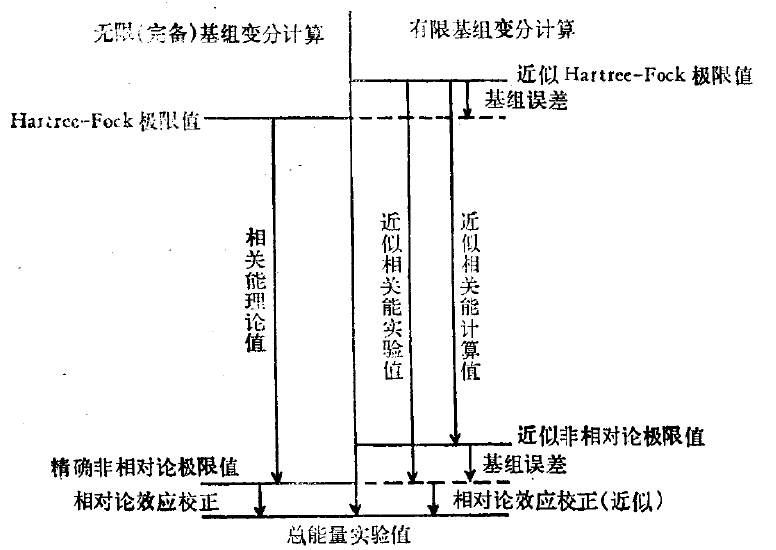
\includegraphics[height=0.42\textwidth,width=0.6\textwidth,viewport=0 0 760 550,clip]{Figures/Post-HF.png}
%\caption{\textrm{ABINIT}的Si.in}
\label{Post-HF}
\end{figure}
}

\frame
{
	\frametitle{Post-HF}
	\textrm{Hartree-Fock}方法精确定义了交换作用,完全没考虑电子相关作用
	\begin{itemize}
		\item \textrm{CI (Configuration Interaction)}
	$$\Psi=\sum_{I=0}C_I\Phi_I=C_0\Phi_0+C_1\Phi_1+C_2\Phi_2+\cdots$$
		\item \textrm{CC (Couple Cluste)}\\
			\begin{displaymath}
				\Psi=\mathrm{e}^{\hat{\mathbf T}}\Phi_0=\mathrm{e}^{(\hat{\mathbf T_1}+\hat{\mathbf T_2}+\hat{\mathbf T_3}+\cdots)}\Phi_0
			\end{displaymath}
		\item \textrm{MP}微扰方法
			\begin{displaymath}
				\begin{aligned}
					&\hat{\mathbf H}=\hat{\mathbf H}^{(0)}+\hat{\mathbf V} \\
					&\hat{\mathbf H}^{(0)}=\sum_i\hat{\mathbf F}_i \qquad \Phi^{(0)}=\Psi_{\mathrm{HF}}\\ 
					&\hat{\mathbf V}=\sum_{j>i}^{occ}\dfrac{e^2}{r_{ij}}-\sum_{ij}^{occ}\big(\hat{\mathbf J}_{ij}-\dfrac12\hat{\mathbf K}_{ij}\big)
				\end{aligned}
			\end{displaymath}
	\end{itemize}
}
%\frame
%{
%\frametitle{发展统一理论框架下的材料计算程序}
%\begin{itemize}
%	\item
%\end{itemize}
%}

\appendix
%------------------------------------------------------------------------Reference----------------------------------------------------------------------------------------------
%\begin{thebibliography}{99}
%-----------------------------------------------------------------------------------------------------------------------------------------------------------------------%
%\frame
%{
%\frametitle{主要参考文献}
%{\small
%\bibitem{Singh_Book}\textrm{D. J. Singh. \textit{Plane Wave, PseudoPotential and the LAPW method} (Kluwer Academic, Boston,USA, 1994)}					%
%  \nocite{*}																				%
%}
%}
%\end{thebibliography}
\begin{thebibliography}{99}
\frame
{
\frametitle{主要参考文献}
{\small
	\bibitem{Xu_Li_Wang}徐光宪、黎乐民、王德民, {\textit{量子化学——基本原理和从头计算法}}\;\textrm{({\textit{上、中}})}\:科学出版社, 北京, 1980
	\bibitem{Elect_Stru}\textrm{Richard. M. Martin. \textit{Electronic Structure: Basic Theory and Practical Methods} (Cambridge University Press, Cambridge, England, 2004)}
}
\nocite*{}
}
\end{thebibliography}
%{\small
%\phantomsection\addcontentsline{toc}{section}{Bibliography}	 %直接调用\addcontentsline命令可能导致超链指向不准确,一般需要在之前调用一次\phantomsection命令加以修正	%
%\bibliography{Myref}																			%
%\bibliographystyle{mybib}																		%
%  \nocite{*}																				%
%}
%-----------------------------------------------------------------------------------------------------------------------------------------------------------------------%


%-----------------------------------------------------------Beamer下不建议使用bib,因为涉及分页--------------------------------------------------------------------------%
%{\small
%\phantomsection\addcontentsline{toc}{section}{Bibliography}	 %直接调用\addcontentsline命令可能导致超链指向不准确,一般需要在之前调用一次\phantomsection命令加以修正	%
%\bibliography{Myref}																			%
%\bibliographystyle{mybib}																		%
%  \nocite{*}																				%
%}

%------------------------------------------------------------------------------------------------------------------------------------------------------------------------------%

%-------------------------------------------------------------------------Thanks------------------------------------------------------------------------------------------------
%\section{致谢}
%\frame
%{
%\frametitle{致$\quad$谢}
%\begin{itemize}
%    \setlength{\itemsep}{20pt}
%  \item 感谢本团队高兴誉、吴泉生、宋红州等各位老师参与的讨论
%  \item 感谢莫所长、宋主任以及软件中心各位老师和同事
%  \item 感谢王崇愚先生的帮助
%\end{itemize}
%}

\logo{}
\frame
{
\vskip 60 pt
%\hskip 10pt \textcolor{blue}{\Huge 感谢答辩委员会各位老师\,\textrm{!}}\\
\vskip 35 pt
\hskip 60pt \textcolor{blue}{\Huge 谢谢大家\:!}
%\vskip 15 pt
%\hskip 40pt \textcolor{blue}{\Huge \textrm{for your attention\:!}}
}

%-------------------------------------------------------------------------------------------------------------------------------------------------------------------------------

\clearpage
%\end{CJK*}
\end{document}
